%-------------------------------------------------------------------------------
\chapter{Quality of Resource Estimation}
\labelchapter{app.resource}

%-------------------------------------------------------------------------------
This Appendix introduces a more detailed version of the histograms of relative differences that were presented in Figure \ref{ch.expe:sec.estimators:ssec.resource:fig.all}.

For each of the considered kernels --- namely {\it Black Scholes}, {\it Pi}, {\it FFT} and {\it Dot Product} --- we exhibit the relative differences of the resource estimations with respect to the synthesis results, for both macro and non-macro estimation methodologies that were introduced in Section \ref{ch.estimators:sec.resource-timing}.
As for the {\it GEMM} kernel, the relative differences are shown in Figure \ref{ch.expe:sec.strategies:ssec.resource:fig.gemm}, as they are used for exploration purposes in Section \ref{ch.expe:sec.strategies:ssec.resource}.

Please refer to Table \ref{ch.expe:sec.estimators:ssec.resource:table.kernels} for both the experimental setups and the temporal considerations of these experiments.

\vspace*{\fill}
\minilof

\clearpage

\clearpage

\begin{figure}[h!]
    \centering
    \begin{subfigure}{1.0\textwidth}
        \centering
        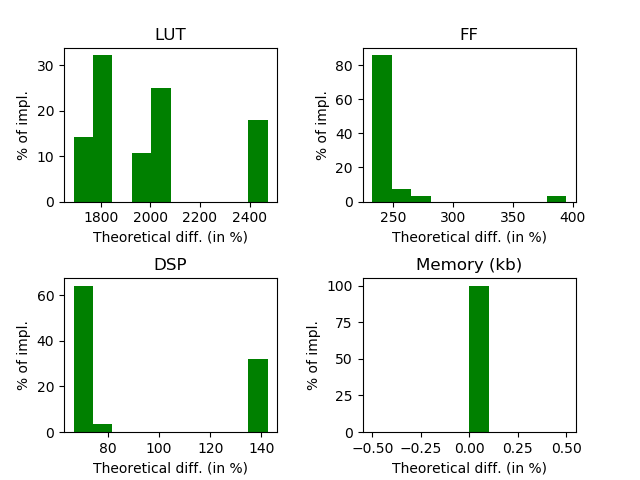
\includegraphics[width=.8\textwidth]{Figures/results/bsRelativeWithoutMacro}
        \caption{Without macro block replacement}
        \label{ch.expe:sec.estimators:ssec.resource:fig.bs:sfig.without}
    \end{subfigure}
    \begin{subfigure}{1.0\textwidth}
        \centering
        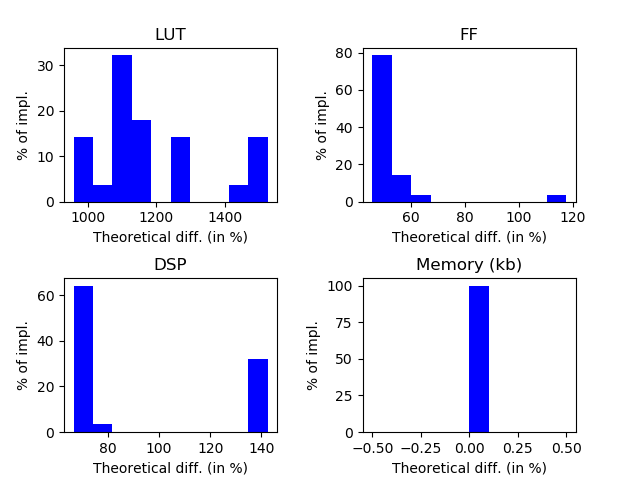
\includegraphics[width=.8\textwidth]{Figures/results/bsRelativeWithMacro}
        \caption{With macro block replacement}
        \label{ch.expe:sec.estimators:ssec.resource:fig.bs:sfig.with}
    \end{subfigure}
    \caption[Quality of resource estimation on Black Scholes]{Relative differences between the resource estimations\newline and the synthesis results on Black Scholes kernels}
    \label{ch.expe:sec.estimators:ssec.resource:fig.bs}
\end{figure}
\clearpage

\begin{figure}[h!]
    \centering
    \begin{subfigure}{1.0\textwidth}
        \centering
        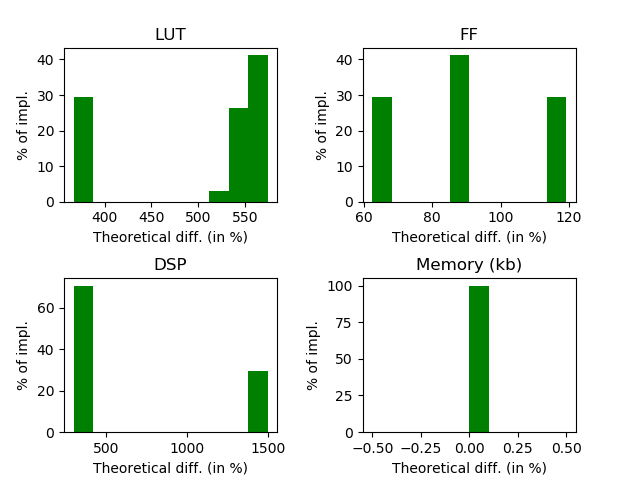
\includegraphics[width=.8\textwidth]{Figures/results/piRelativeWithoutMacro}
        \caption{Without macro block replacement}
        \label{ch.expe:sec.estimators:ssec.resource:fig.pi:sfig.without}
    \end{subfigure}
    \begin{subfigure}{1.0\textwidth}
        \centering
        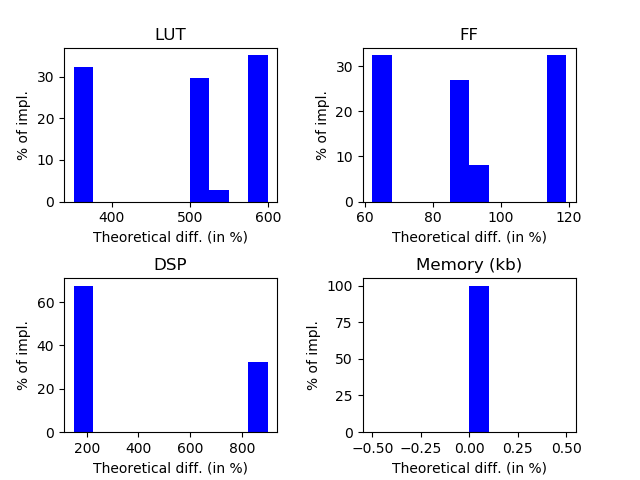
\includegraphics[width=.8\textwidth]{Figures/results/piRelativeWithMacro}
        \caption{With macro block replacement}
        \label{ch.expe:sec.estimators:ssec.resource:fig.pi:sfig.with}
    \end{subfigure}
    \caption[Quality of resource estimation on Pi]{Relative differences between the resource estimations\newline and the synthesis results on Pi kernels}
    \label{ch.expe:sec.estimators:ssec.resource:fig.pi}
\end{figure}
\clearpage

\begin{figure}[h!]
    \centering
    \begin{subfigure}{1.0\textwidth}
        \centering
        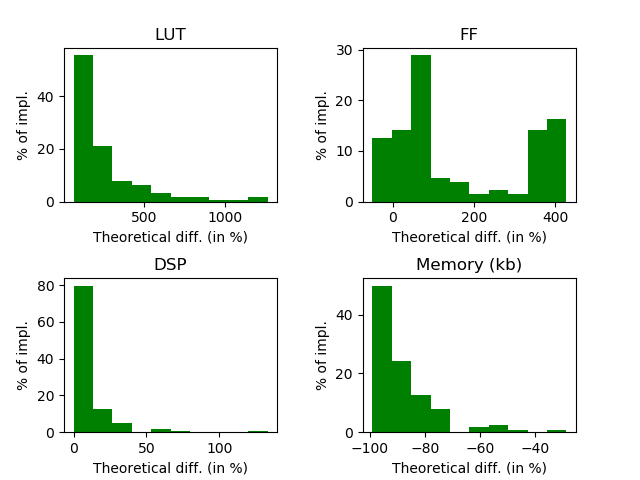
\includegraphics[width=.8\textwidth]{Figures/results/fftRelativeWithoutMacro}
        \caption{Without macro block replacement}
        \label{ch.expe:sec.estimators:ssec.resource:fig.fft:sfig.without}
    \end{subfigure}
    \begin{subfigure}{1.0\textwidth}
        \centering
        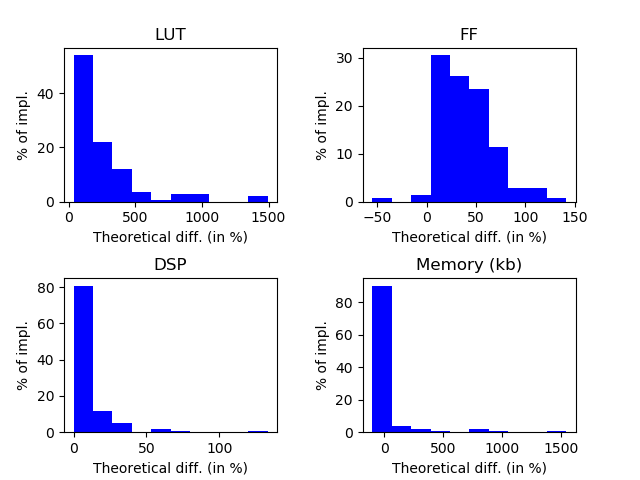
\includegraphics[width=.8\textwidth]{Figures/results/fftRelativeWithMacro}
        \caption{With macro block replacement}
        \label{ch.expe:sec.estimators:ssec.resource:fig.fft:sfig.with}
    \end{subfigure}
    \caption[Quality of resource estimation on FFT]{Relative differences between the resource estimations and\newline the synthesis results on Fast-Fourier Transform kernels}
    \label{ch.expe:sec.estimators:ssec.resource:fig.fft}
\end{figure}
\clearpage

\begin{figure}[h!]
    \centering
    \begin{subfigure}{1.0\textwidth}
        \centering
        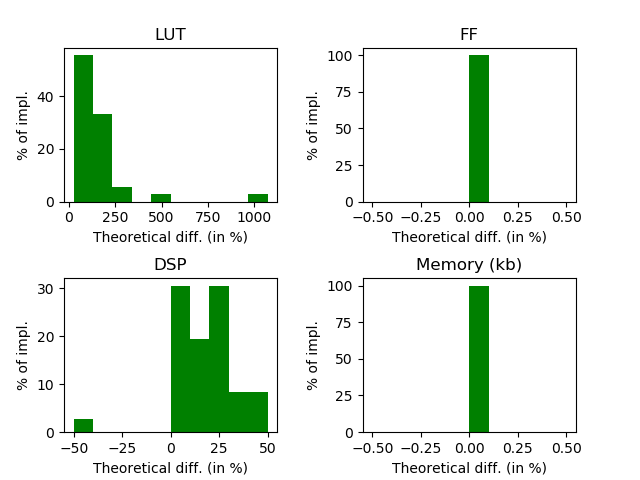
\includegraphics[width=.8\textwidth]{Figures/results/dpRelativeWithoutMacro}
        \caption{Without macro block replacement}
        \label{ch.expe:sec.estimators:ssec.resource:fig.dp:sfig.without}
    \end{subfigure}
    \begin{subfigure}{1.0\textwidth}
        \centering
        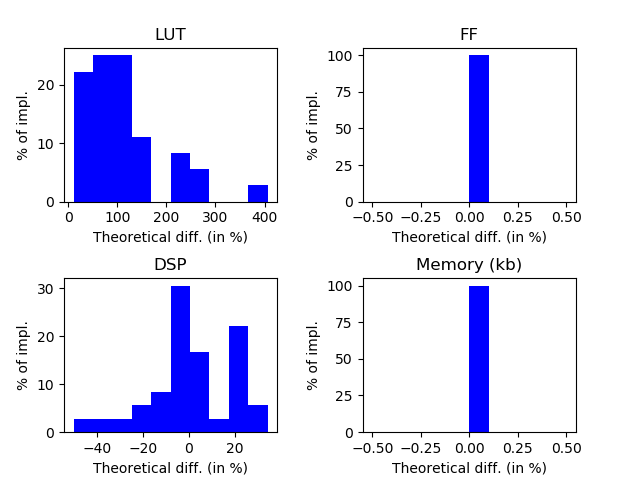
\includegraphics[width=.8\textwidth]{Figures/results/dpRelativeWithMacro}
        \caption{With macro block replacement}
        \label{ch.expe:sec.estimators:ssec.resource:fig.dp:sfig.with}
    \end{subfigure}
    \caption[Quality of resource estimation on dot product]{Relative differences between the resource estimations and\newline the synthesis results on dot product kernels}
    \label{ch.expe:sec.estimators:ssec.resource:fig.dp}
\end{figure}
\clearpage
